\section{Modelling}

\begin{frame}{Scheme of MLS system}

    \begin{figure}[H]

        \begin{minipage}{0.40\textwidth}

            \centering

            \begin{tikzpicture}[european voltages]

                \def\radius{0.3}

                % Upper circuit
                \node at (-1.0, 3.5) {$T_1$};
                \draw (-3, 3.5) node [right] {$+$}
                to [short] ++(0, -1)
                to [R, l^=$R_1$, resistors/zigs=6] ++(2, 0)
                to [variable cute inductor, i>^=$I_1$, l=$L_1$] ++(2, 0)
                to [short] ++(0, +1) node [right] {$-$};

                % Reference system
                \draw[|->] (-1.0, +2.5) -- ++(0, -3) node[left] {$z$, $\dot{z}$, $\ddot{z}$};

                % Ball
                \filldraw[fill=gray, draw=black] (0, 0) circle (\radius);

                % Upward forces
                \draw[thick, ->] (-0.1, +\radius) -- ++(0, +1.5) node[right] {$F_{\text{em1}}$};
                \draw[thick, ->] (+0.0, +\radius) -- ++(0, +1.0) node[right] {$F_{\text{in}}$};
                \draw[thick, ->] (+0.1, +\radius) -- ++(0, +0.5) node[right] {$F_{\text{d}}$};

                % Downward forces
                \draw[thick, ->] (+0.1, -\radius) -- ++(0, -0.5) node[right] {$F_{\text{g}}$};
                \draw[thick, ->] (-0.1, -\radius) -- ++(0, -1.0) node[right] {$F_{\text{em2}}$};

                % Lower circuit
                \node at (-1.0, -3.0) {$T_2$};
                \draw (-3, -3) node [right] {$+$}
                to [short] ++(0, +1)
                to [R, l_=$R_2$, resistors/zigs=6] ++(2, 0)
                to [variable cute inductor, i>_=$I_2$, l_=$L_2$] ++(2, 0)
                to [short] ++(0, -1) node [right] {$-$};

            \end{tikzpicture}

        \end{minipage}
        %
        \hfill
        %
        \begin{minipage}{0.55\textwidth}

            \centering

            \begin{tabular}{|c|l|c|}
                \hline
                \textbf{Name}      & \textbf{Description}               & \textbf{Units} \\
                \hline
                $F_{\text{g}}$     & Gravitational force                & N              \\
                $F_{\text{in}}$    & Inertial force                     & N              \\
                $F_{\text{d}}$     & Drag force                         & N              \\
                $F_{\text{em1,2}}$ & Electromagnetic forces             & N              \\
                \hline
                $R_{1,2}$          & Resistances of the coils           & $\Omega$       \\
                $L_{1,2}$          & Inductances of the coils           & H              \\
                $I_{1,2}$          & Currents flowing through the coils & A              \\
                $V_{1,2}$          & Voltages applied to the coils      & V              \\
                $T_{1,2}$          & Temperatures of the coils          & $^\circ C$     \\
                \hline
            \end{tabular}

        \end{minipage}

        \label{fig:MLS_scheme}

    \end{figure}

\end{frame}



\begin{frame}{Equations of motion}

    We started from the Lagrange equation of the system and we derived the \textbf{equations of motion}.

    \begin{equation}
        \frac{d}{dt} \left( \frac{\partial \mathcal{T}}{\partial \dot{\mathbf{u}}} \right) - \frac{\partial \mathcal{T}}{\partial \mathbf{u}} + \frac{\partial \mathcal{D}}{\partial \dot{\mathbf{u}}} + \frac{\partial \mathcal{U}}{\partial \mathbf{u}} = \mathcal{Q}
        \label{eq:lagrange_equation}
    \end{equation}

    Where the energy terms are defined as follows:

    \begin{equation}
        \begin{aligned}
            \mathcal{T} & = \frac{1}{2} m \dot{z}^2 + \frac{1}{2} L_1(z, \dot{q_1}) \dot{q_1}^2 + \frac{1}{2} L_2(z, \dot{q_2}) \dot{q_2}^2                                                                             \\
            \mathcal{D} & = \int_{\dot{z}(\cdot)} \frac{1}{2} C_d A \rho \dot{z}^2 d\dot{z} + \int_{\dot{q_1}(\cdot)} R_1(\dot{q_1}) \dot{q_1} d\dot{q_1} + \int_{\dot{q_2}(\cdot)} R_2(\dot{q_2}) \dot{q_2} d\dot{q_2} \\
            \mathcal{U} & = -m g z - q_1 V_1 - q_2 V_2                                                                                                                                                                  \\
            \mathcal{Q} & = 0
        \end{aligned}
    \end{equation}

\end{frame}



\begin{frame}{Electrical components model}

    From experimental data, we have proposed a model for both the resistances and the inductances of the coils.

    \begin{equation}
        \begin{aligned}
            R_1 & = R_1(\dot{q_1}, T_1) = R_{10} \\
            R_2 & = R_2(\dot{q_2}, T_2) = R_{20}
        \end{aligned}
        \label{eq:model_for_resistance}
    \end{equation}

    \begin{equation}
        \begin{aligned}
            L_1 & = L_1(z, \dot{q_1}, T_1) = L_{10} + L_{1z} e^{-a_{1z} z} + L_{1I} * \arctan(a_{1I} I_{1} - b_{1I})            \\
            L_2 & = L_2(z, \dot{q_2}, T_2) = L_{20} + L_{2z} e^{-a_{2z} (h - 2r - z)} + L_{2I} * \arctan(a_{2I} I_{2} - b_{2I})
        \end{aligned}
        \label{eq:model_for_inductance}
    \end{equation}

\end{frame}



\begin{frame}{Model reduction}

    In order to simplify the model, we have \textbf{neglected the effect of the current on the value of the inductances (strong assumption)}.
    We also have neglected any velocity linearly dependent terms in the equations of motion.

    \begin{equation}
        \begin{cases}
            \frac{\partial L}{\partial I}     & \approx 0 \\
            \frac{\partial^2 L}{\partial I^2} & \approx 0 \\
            \dot{z}                           & \approx 0
        \end{cases}
        \label{eq:model_reduction_conditions}
    \end{equation}

\end{frame}



\begin{frame}{Equations of motion (single coil configuration)}

    We decided to focus on the \textbf{single coil configuration}, considering the MLS as a SISO system.

    \begin{equation}
        \begin{cases}
            \dot{z} = v                                                                                                                                 \\
            \dot{v} = m^{-1} \left(\frac{1}{2} \frac{\partial L_1}{\partial z} I_1^2 + \frac{1}{2} \frac{\partial L_2}{\partial z} I_2^2 + m g  \right) \\
            \dot{I_1} = L_1^{-1} \left(- R_1 I_1 + (k_1 U_1 + c_1) \right)                                                                              \\
            \dot{I_2} = L_2^{-1} \left(- R_2 I_2 + (k_2 U_2 + c_2) \right)
        \end{cases}
        \label{eq:reduced_quations_of_motion_final}
    \end{equation}

    Despite tge simplification applied with Equation \ref{eq:model_reduction_conditions}, the model is still \textbf{able to capture the main dynamics of the system}.

\end{frame}



\begin{frame}{Linearization and state-space form}

    We have linearized the system around the equilibrium point $(z_{op}, v_{op}, I_{1op})$, computed by nullifying the right-hand side of Equation \ref{eq:reduced_quations_of_motion_final} and derived also the state-space form.

    \vspace{9pt}

    Full derivation of the linearized system is available in the report.

\end{frame}

\begin{frame}{Controlling}

    \only<1>{
        We have implemented a Simulink model of the system.

        \begin{figure}
            \centering
            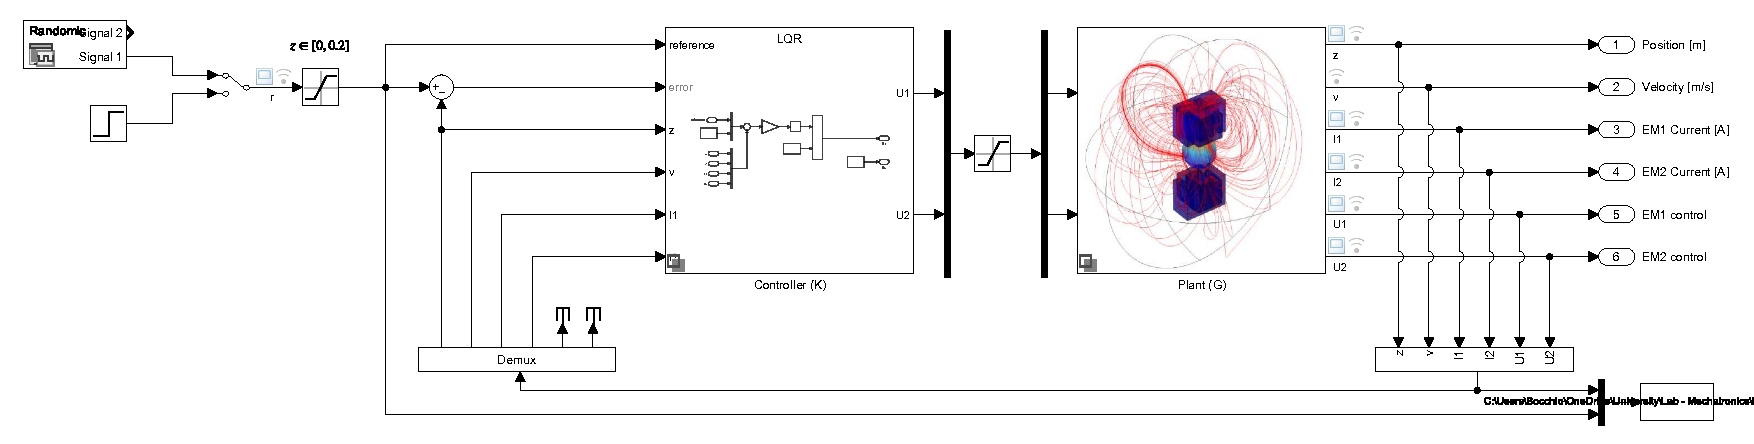
\includegraphics[width=1\textwidth]{img/MATLAB/simulink_model.pdf}
            \caption{Simulink root model of the Magnetic Levitation System}
        \end{figure}

        Some controllers have also been implemented and tested.

    }

    \only<2>{
        PID (both with and without anti-windup) controllers have been tested.

        \begin{figure}
            \centering
            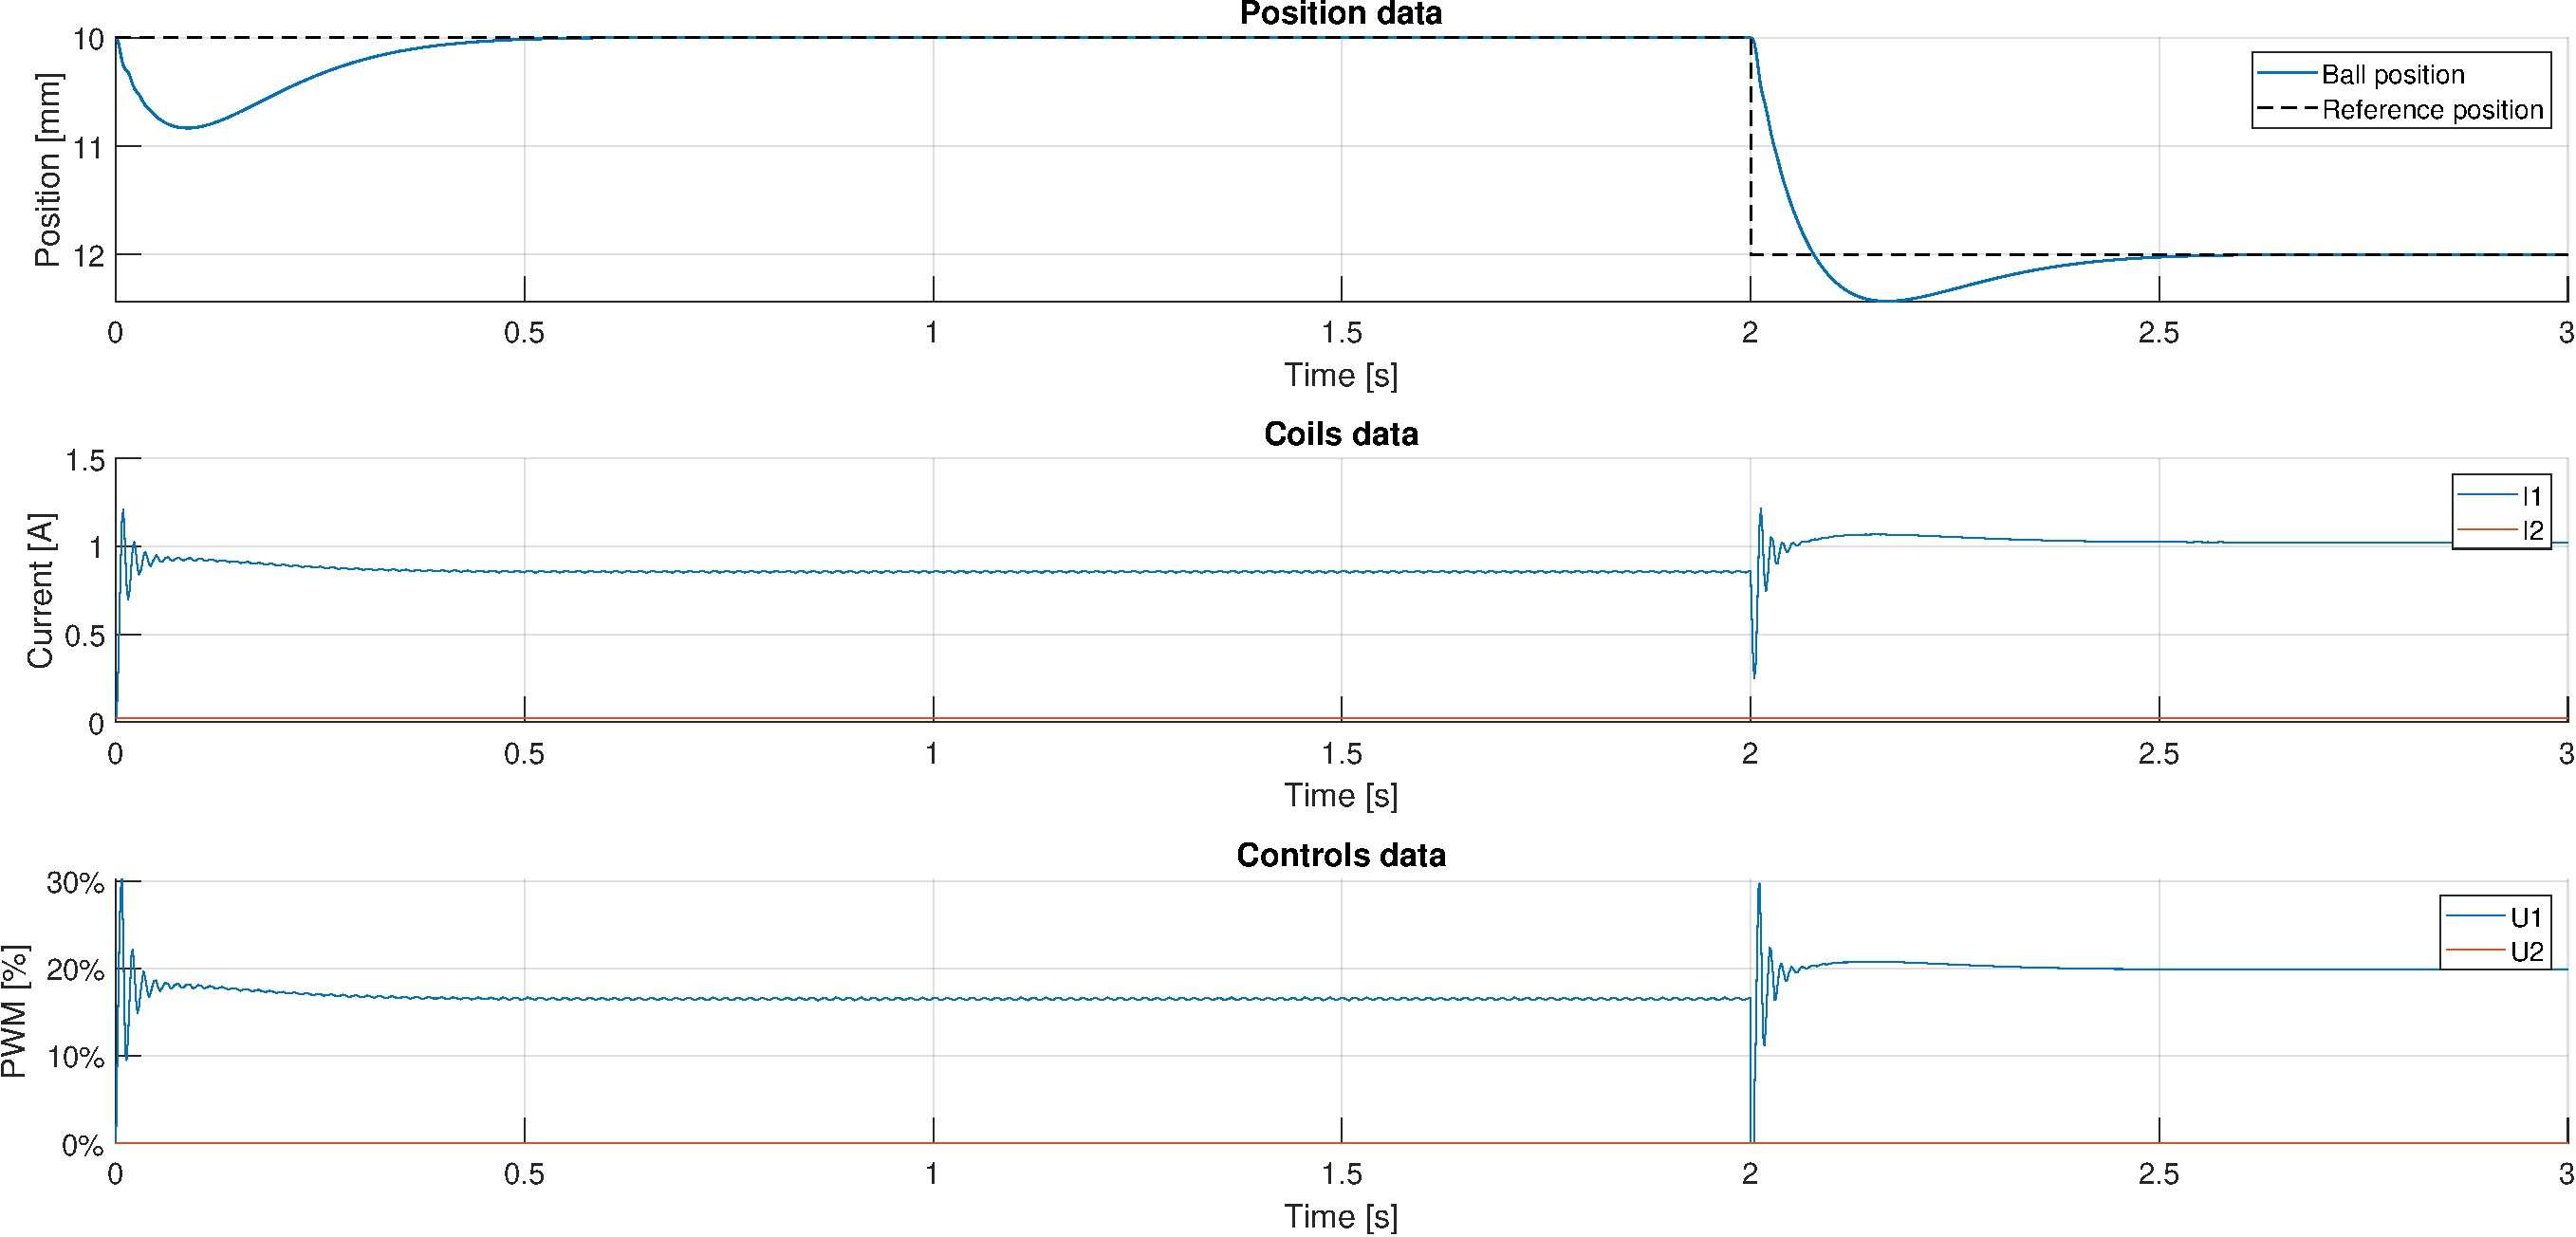
\includegraphics[width=1\textwidth]{img/MATLAB/runs/PID_anti_windup.pdf}
            \caption{PID with anti-windup controller}
        \end{figure}

        A PID controller without anti-windup has also been tested but with a clearly worse performance (strong oscillations around the reference).

    }

    \only<3>{
        LQR controllers with (limited) tracking capabilities have been tested.

        \begin{figure}
            \centering
            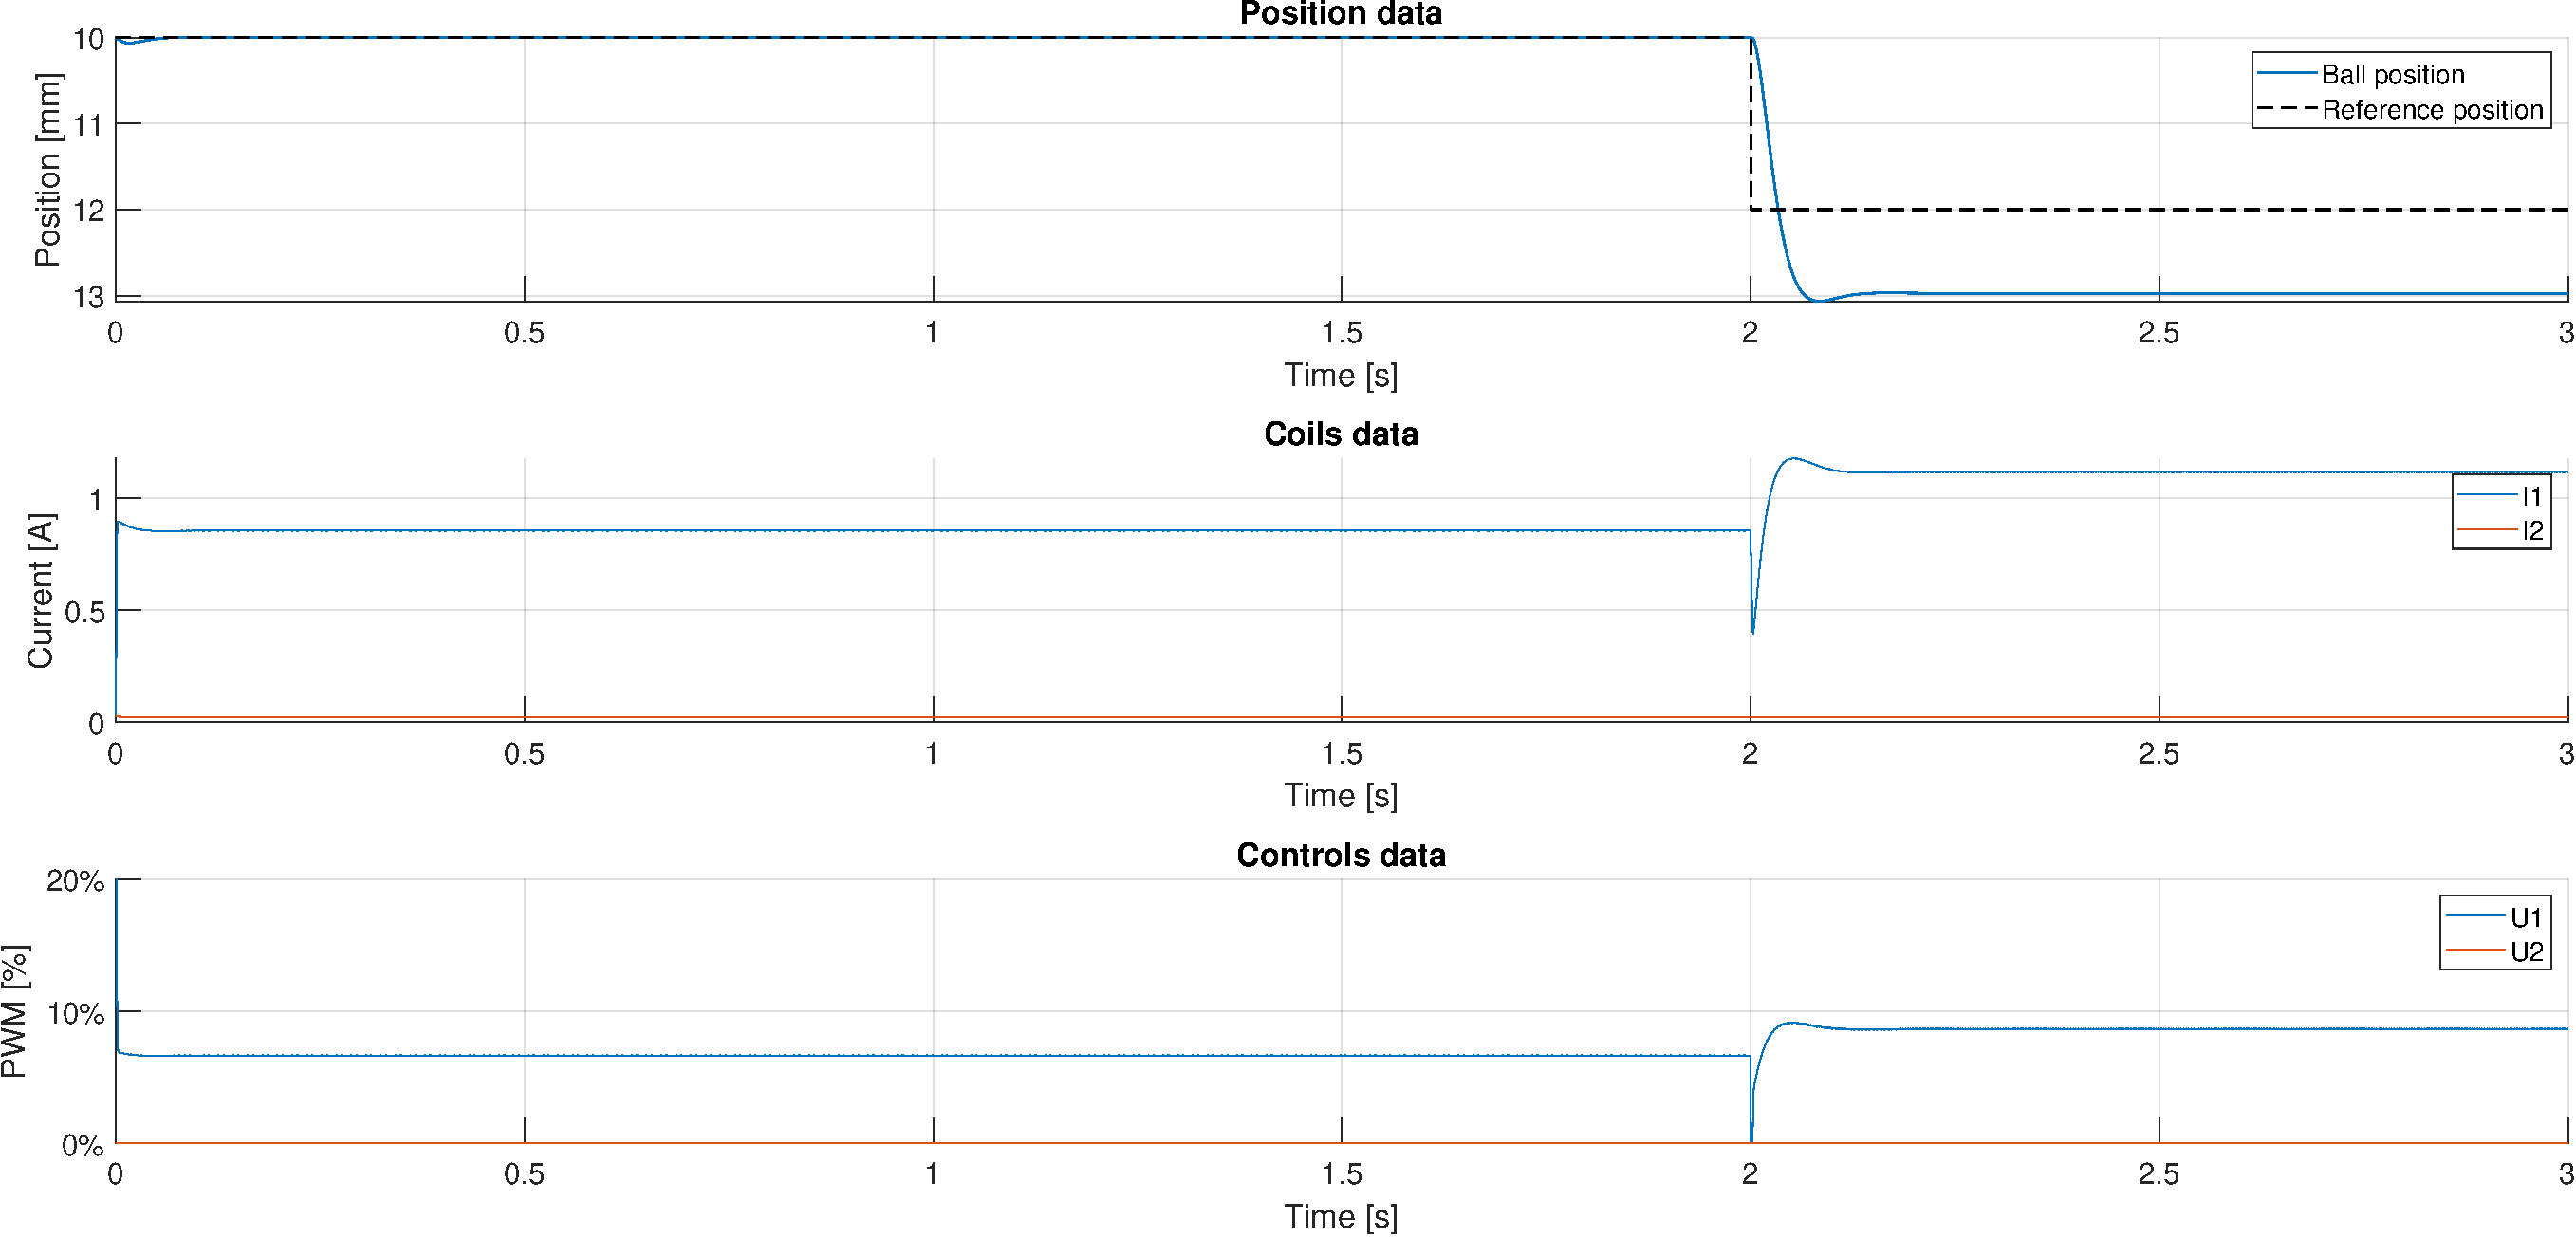
\includegraphics[width=1\textwidth]{img/MATLAB/runs/LQR_tracking.pdf}
            \caption{LQR controller}
        \end{figure}

    }

\end{frame}

